\newcommand\abs[1]{\ensuremath{\lvert #1 \rvert}}

\subsection{3-Clique merge}

\subsubsection*{Description}

In this experiment we find all the 3-cliqes~\cite{wiki_clique} (triangles) in the graph, then sort them based on `distance' and replace each 3-clique with one node sharing the features of the initial three.

The source code is available in the project repository and can be found in the `experiments' directory~\cite{3clique_experiment}.

\subsubsection*{Algorithm}

Firstly, let us define a 3-clique more formally.
We define it as follows: $
\{ \left(a, b, c\right)\ 
\lvert\ a, b, c \in V \wedge
\left(a, b\right),
\left(a, c\right),
\left(b, c\right) \in E \} $.

While merging nodes in the cliques, we might face a problem: some of the nodes might participate in several 3-cliques.
In order to solve it, we need to introduce a mechanism for ordering cliques so that we could show preference to one instead of the other.
Naturally, such a mechanism should rely on the nodes feature vectors.
There are 2 major distance calculating algorithms: Euclidean distance and Manhattan distance.
Since the feature vectors are very sparse, the algorithms give quite close results and there is no need to consider them separately.

Using Euclidean distance we can map each 3-clique into a real number by calculating the sum of pairwise distances: $\abs{a_f - b_f}^2 + \abs{a_f - c_f}^2 + \abs{b_f - c_f}^2$, where $v_f$ stands for node's $v$ feature vector.
The resulting ordering now allows us to choose one 3-clique instead of another, since we know that one has its nodes `closer' to each other.

Therefore, one can simply sort all the 3-cliques in ascending order, merge each 3-clique and filter out all the `later' 3-cliques containing nodes from the current one.
This allows us pick the closest and most valuable nodes in a greedy way while also saving us from using a `new' node in another 3-clique ($(a, b, c) \rightarrow a';\ (a', d, e) \rightarrow a''$ is not allowed, since the graph could collapse).

\begin{enumerate}
    \item Find all the 3-cliques in graph.
    \item Sort them according to the sum of distances between nodes
    \item Merge all `valid' 3-cliques in one node preserving all the edges coming in and out of the triplet filtering out all the cliques containing nodes from the merged ones
    \item Generate new dataset from the resulting graph
\end{enumerate}

\subsubsection*{Results and interpretation of them}

A benchmark on the Cora dataset~\cite{cora_dataset} had shown that we are able to remove a total of 12.2\% of nodes (the number reduced from 2708 to 2378) and 42.3\% edges (from 10556 to 6094).
Since the operation of merging of all cliques fast comparing to the model's learning time, we reduced the latter approximately by 23\%.
This improvement can be also seen on the loss graph of our models:

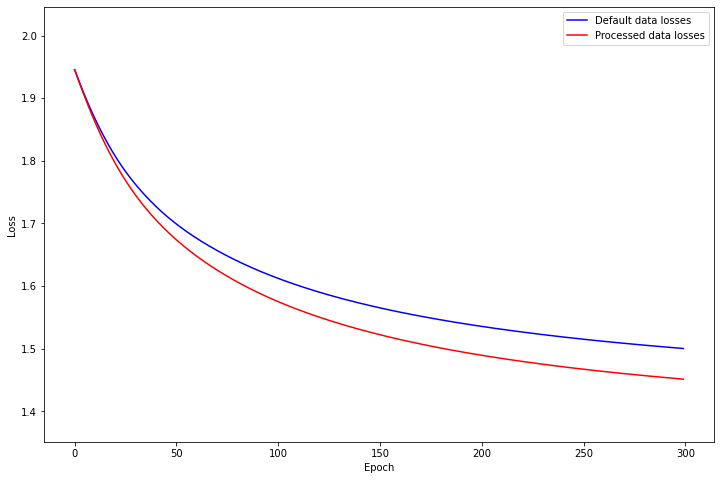
\includegraphics[width=0.9\textwidth]{3clique_loss.png}

Speaking of accuracy, we claim it did not change much.
On average, the accuracy of a default model lies somewhere between 0.7 and 0.75 and the model with 3-cliques merged performs practically same with an error of $\pm 0.005$ (for example, 0.725 vs 0.72402).

Therefore, we can claim that the only purpose of merging 3-cliques is reducing the learning time without any loss of accuracy.
It doesn't make much sense for theoretical purposes, however, is definitely an advantage in production.
